
\documentclass[runningheads]{llncs}
\usepackage[text={150mm,220mm},centering]{geometry}
\usepackage{graphicx}
\usepackage{tikz}
\usepackage{float}
\begin{document}
\title{\large{CSCI814 IT Project Management (Lab1)}}
%--------------------Please do NOT change the content above.-------------------------------------------------

%
%----Please write your personal information as below.------------------------------------
%
\author{\large{Student Name: Wangzhihui Mei \\ % Please write your name here
CCNU Student Number: 2019124044 \\ % Please write your CCNU student number here
UOW Student Number: 6603385}}  % Please write your UOW student number here


%-----------------------------------------------------------------------------------------------



%---------Do not change the content of this part--------------------

\authorrunning{CCNU Wollongong Joint Institute}
\institute{Central China Normal University Wollongong Joint Institute}

\maketitle


%-----------Please write your solutions to the questions in the assignment from here.---------------

\section{In-class exercise}

\begin{figure}[H]
    \centering
    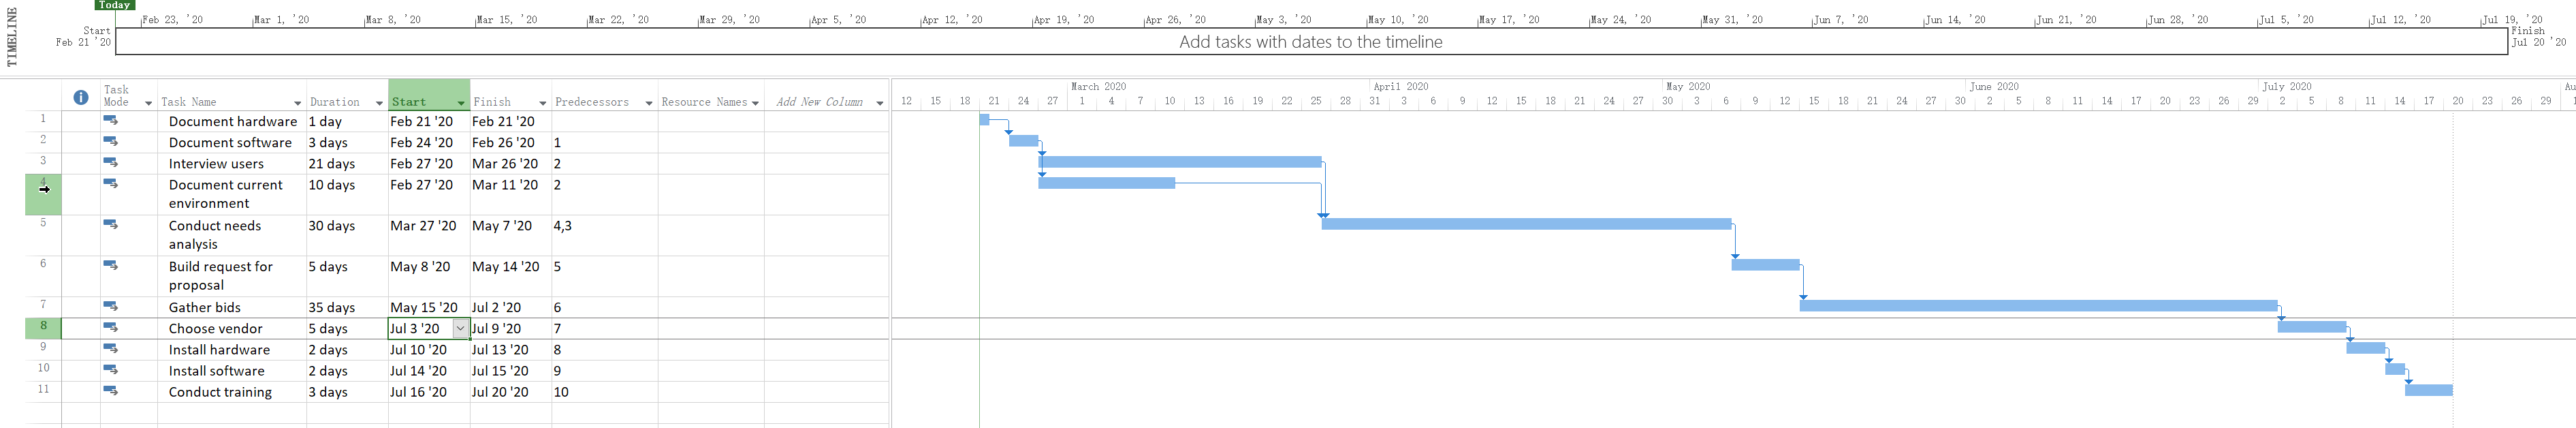
\includegraphics[width=1.0\textwidth]{./image/proj1}
    \caption{Gantt Chart 1}
\end{figure}

\noindent2) The former tasks are the prerequisite of the following tasks.

\noindent3) Timeline: Feb. 21 - Jul. 20, 151 days in total (considering weekends)

\noindent4) Jul. 16, The 147th day of the project

\noindent5) It won't affect the project completion date

\noindent6) Jul. 23, an additional weekend will be included in the timeline.

\noindent7,8,9,10) 
\begin{figure}[H]
    \centering
    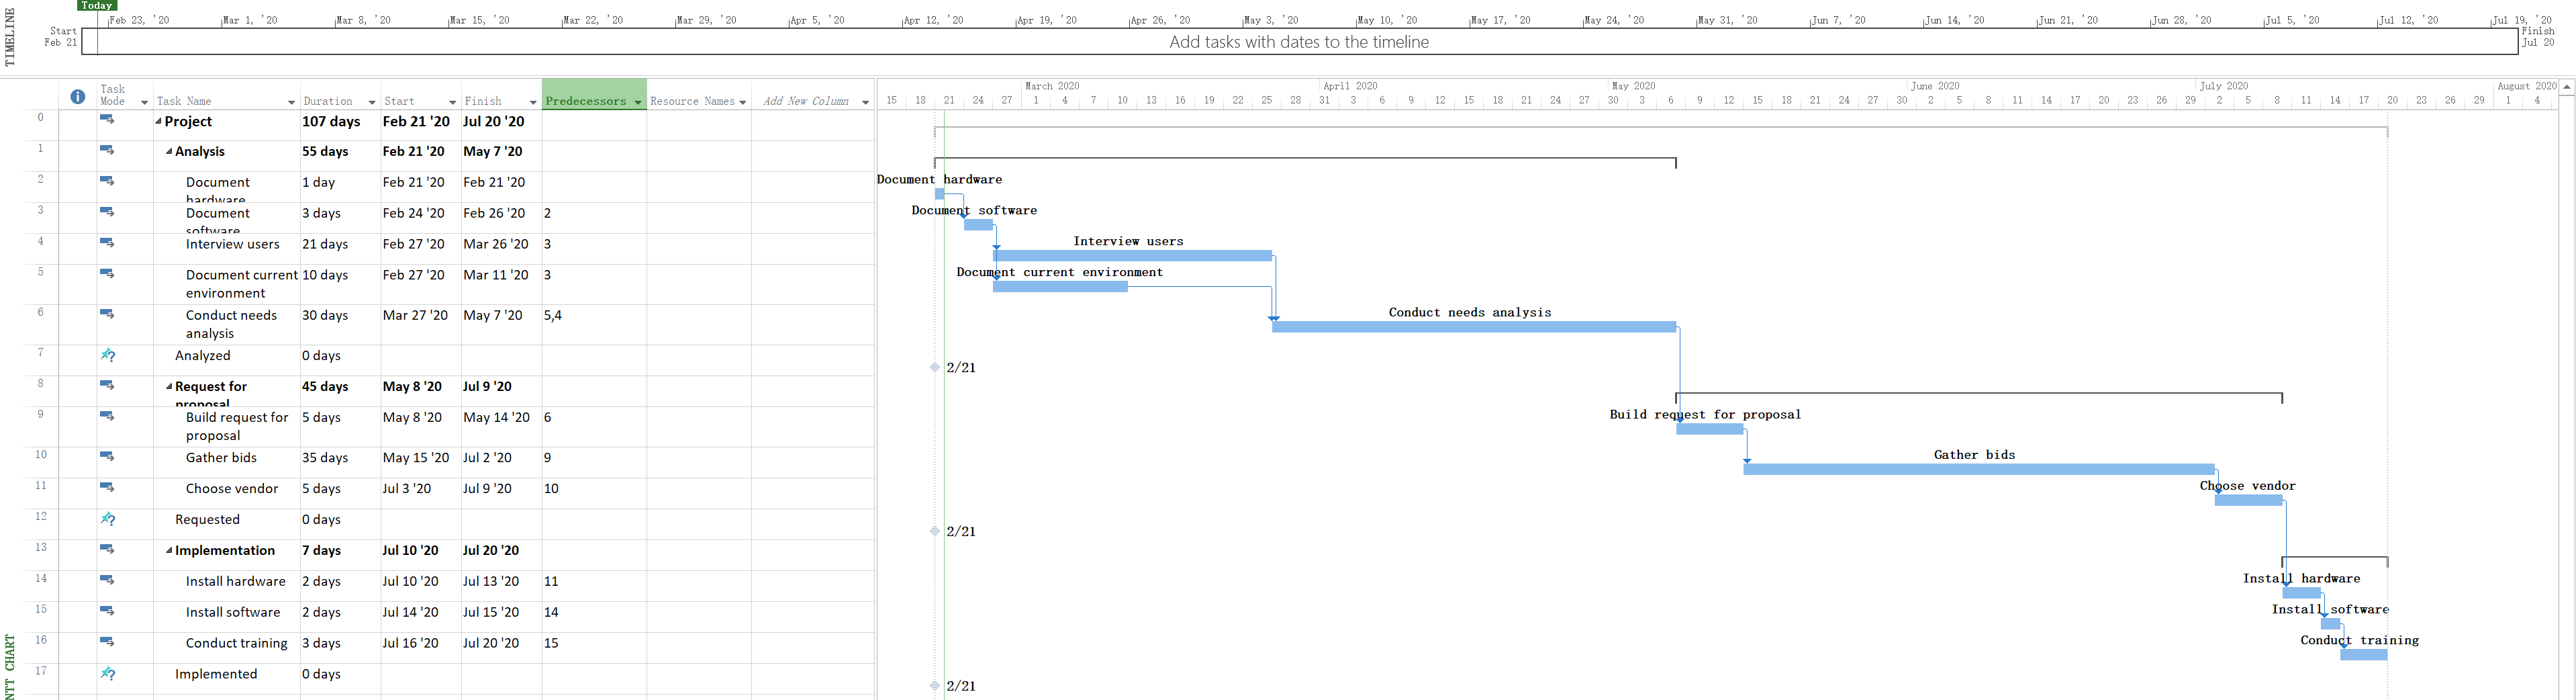
\includegraphics[width=1.0\textwidth]{./image/proj2}
    \caption{Gantt Chart 2}
\end{figure}

\noindent11) Considering Qingming Festival (Apr. 4–6), Labor Day(May 1–5) and The Dragon Boat Festival (June 25–27), the end time will delay to Jul. 28.
\begin{figure}[H]
    \centering
    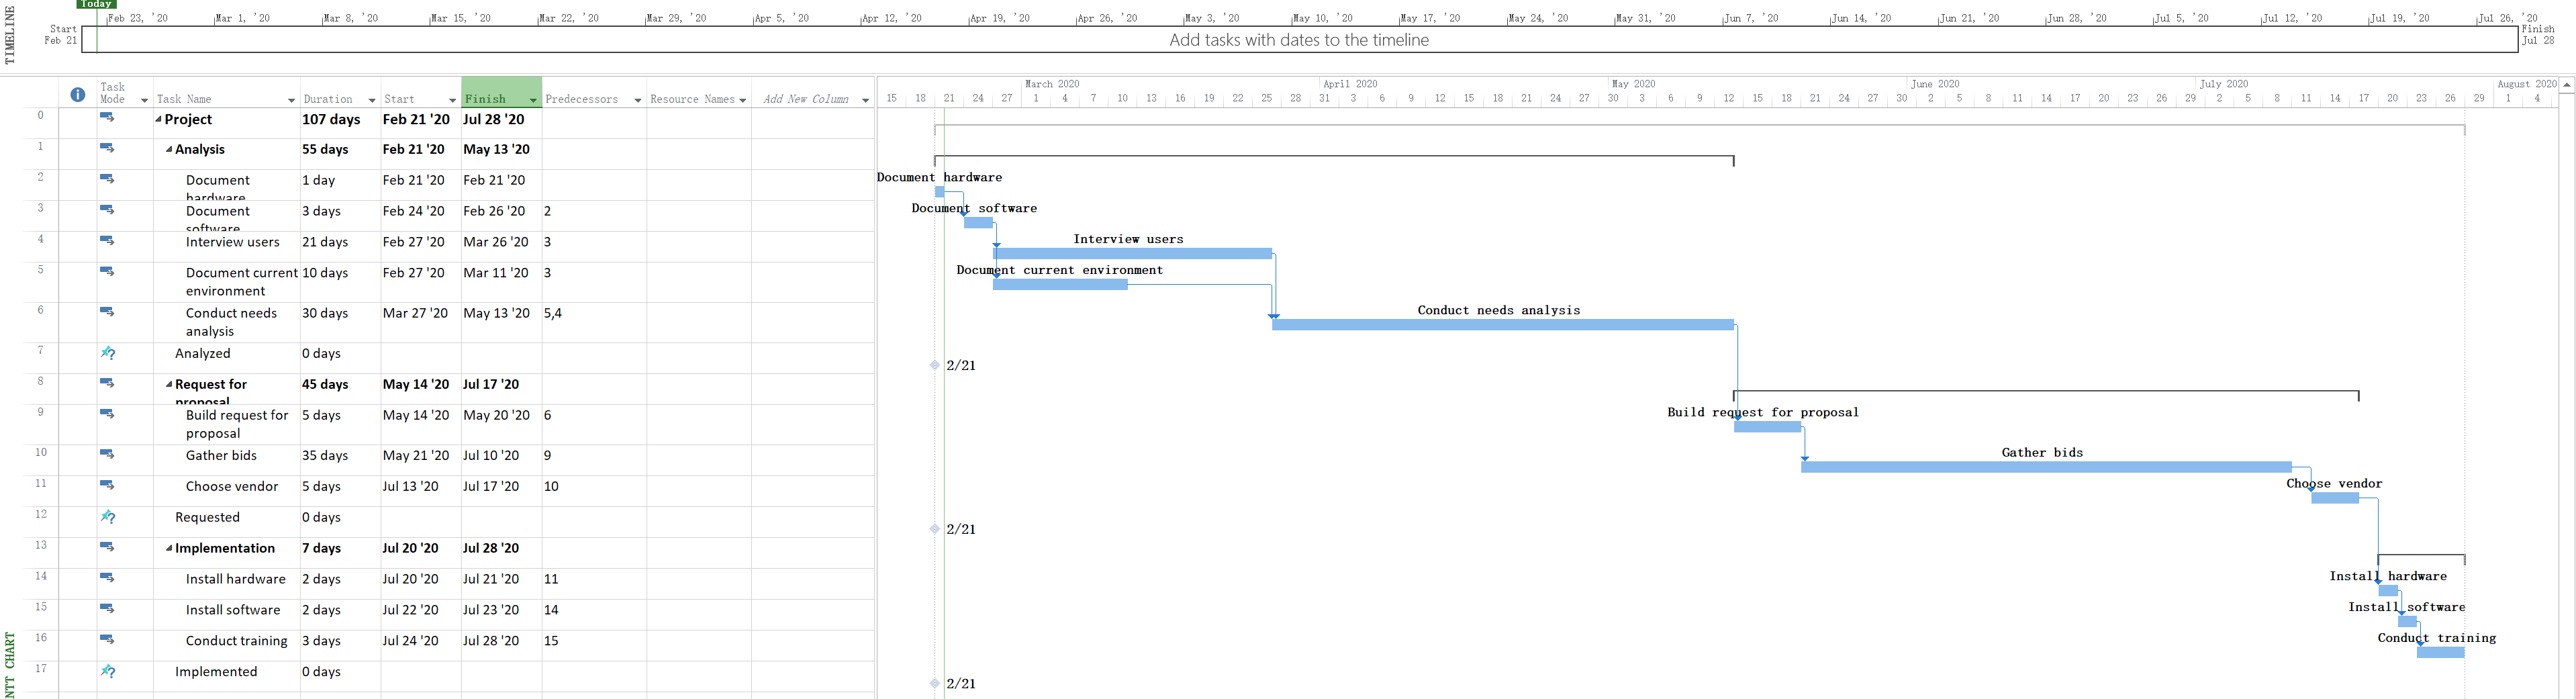
\includegraphics[width=1.0\textwidth]{./image/proj3}
    \caption{Gantt Chart 2}
\end{figure}


\section{Lab1}
\subsection{}


\end{document}
